% Minimal TikZ standalone example

\documentclass[tikz, border=1mm]{standalone}

\usepackage{amsmath,amssymb}
\usepackage{tikz}

\usetikzlibrary{calc,angles,quotes}

\begin{document}

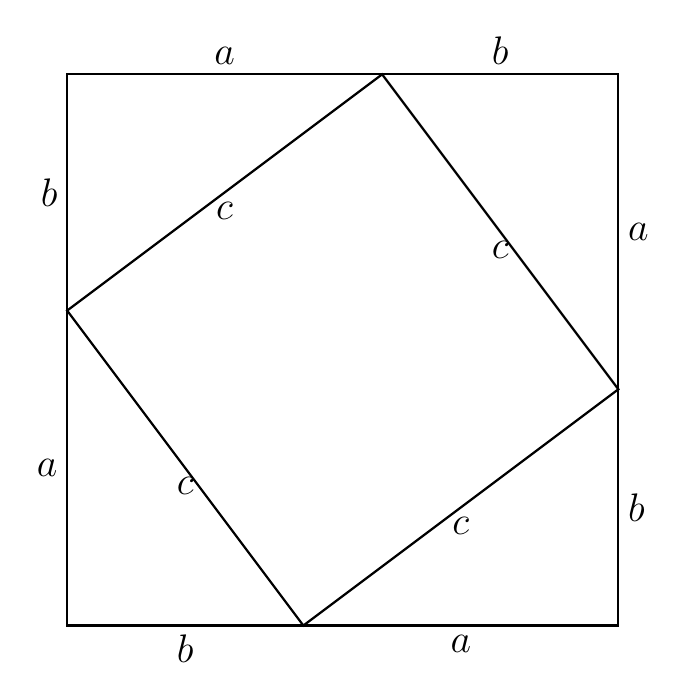
\begin{tikzpicture}[scale=1.0,font=\Large]

	% dots coordinates
	\coordinate (A) at (0,0);
	\coordinate (B) at (7,0);
	\coordinate (C) at (0,7);
	\coordinate (D) at (7,7);

	\coordinate (E) at (3,0);
	\coordinate (F) at (7,3);
	\coordinate (G) at (4,7);
	\coordinate (H) at (0,4);

	% squares and triangles
	\draw[thick] (0,0) rectangle (7,7);
	\draw[thick] (E)--(F)--(G)--(H)--cycle;

	% edges labels
	\node[below] at ($(E)!0.5!(F)$) {$c$};
	\node[below] at ($(F)!0.5!(G)$) {$c$};
	\node[below] at ($(G)!0.5!(H)$) {$c$};
	\node[below] at ($(H)!0.5!(E)$) {$c$};

	\node[below] at ($(A)!0.5!(E)$) {$b$};
	\node[below] at ($(E)!0.5!(B)$) {$a$};

	\node[right] at ($(B)!0.5!(F)$) {$b$};
	\node[right] at ($(F)!0.5!(D)$) {$a$};

	\node[above] at ($(D)!0.5!(G)$) {$b$};
	\node[above] at ($(G)!0.5!(C)$) {$a$};

	\node[left] at ($(C)!0.5!(H)$) {$b$};
	\node[left] at ($(H)!0.5!(A)$) {$a$};
\end{tikzpicture}

\end{document}
